\subsection{Scribe}
\label{chap:related:scribe}
Scribe \cite{Castro2002Scribe} selbst setzt auf dem strukturierten Overlay-Netzwerk Pastry \cite{Rowstron2001} auf und erzeugt einen vom Subscriber zum Publisher aufgebauten \emph{reverse path forwarding tree} \cite{Dalal1978}. Diese Struktur wird Multicast-Tree\index{Multicast-Tree} genannt. Pro Kanal erzeugt Scribe einen eigenen Multicast-Tree.

\begin{figure}[htbp]
\centering
\resizebox{\textwidth}{!}{%
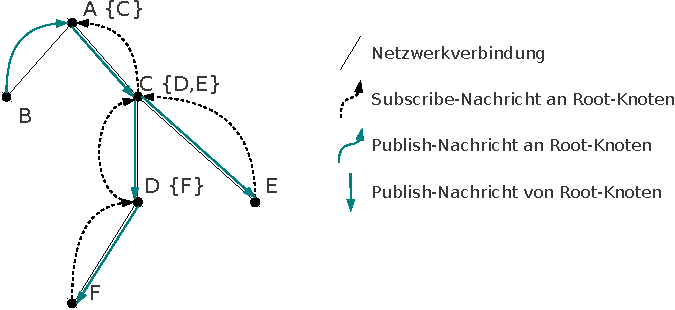
\includegraphics{grafics/multicast_tree.pdf}}
\caption{Schema eines Multicast-Trees}
\label{fig:multicast_tree}
\end{figure}

\Fref{fig:multicast_tree} zeigt ein Netzwerk mit den sechs Knoten A-F. Die Verbindungen der Knoten werden durch dünne schwarze Linien dargestellt. Beispielsweise hat Knoten C Verbindungen zu A, B, D und F. Ein Multicast-Tree benötigt einen Knoten, der die Wurzel (im Folgenden \emph{Root-Knoten} genannt) darstellt. Scribe errechnet aus dem Hashwert des Kanalnamens einen Schlüssel. Derjenige Knoten, der aufgrund der Netzwerkmetrik für diesen Schlüssel zuständig ist, wird Root-Knoten des Kanals. Im abgebildeten Falle ist dies Knoten A. Weiterhin hält jeder Knoten eine Liste bei ihm angemeldeter Knoten. In der Abbildung wird diese Liste durch geschweifte Klammern nach der Knotenbezeichnung dargestellt.

\paragraph{Subscribe}
Zur Anmeldung sendet Knoten F eine \emph{Subscribe}-Nachricht an A. Diese Nachrichten sind in der Grafik durch gebogene gestrichelte schwarze Verbindungslinien mit Pfeil dargestellt. Das Netzwerk würde diese Nachricht über Knoten D und C an A routen. Da Pastry ein Verarbeitungsmodell besitzt, das der generischen \ac{kbr} API entspricht, wird an allen Knoten auf dem Weg von D nach A \texttt{forward} aufgerufen und Scribe kann die Nachricht verändern. Auf Knoten D wird der Sender der Nachricht, Knoten F, in die Liste der Subscriber eingetragen. Die Nachricht wird so verändert, dass Knoten D als Sender eingetragen wird. Somit meldet sich Knoten D selbst am Kanal an. Auf Knoten C wird ähnlich verfahren und D in die Liste eingetragen. A erhält letztlich die Subscribe-Nachricht, liest C als Sender aus und trägt C in die Liste ein.\\
Wenn sich Knoten E für den Kanal einschreibt, wird die Subscribe-Nachricht an A wieder über den Knoten C geleitet. Wieder wird der Sender, Knoten E, in die Liste eingetragen. Da C selbst angemeldet ist, wird die Nachricht terminiert und nicht weiter verschickt.

Scribe fordert periodische Anmeldungen der Knoten um eventuelle Knotenausfälle und die damit einhergehende Unterbrechung des Multicast-Trees zu reparieren. Im Beispiel würden sich E und F nach einem Zeitintervall erneut am Kanal anmelden. Wäre in der Zwischenzeit ein Knoten auf dem Weg zu A ausgefallen, würde die Nachricht über einen anderen Knoten (in der Grafik nicht dargestellt) übertragen werden und sich der Multicast-Tree wieder aufbauen. Knoten, die wie C und D, über den Umweg der Weiterleitung angemeldet sind, können die periodisch ankommenden Subscribe-Nachrichten nutzen, um ihre eigene Anmeldung zu erneuern. Nach einem entsprechenden Zeitintervall würde C die Nachricht von E nicht terminieren sondern sich selbst erneut als Sender eintragen.

\paragraph{Unsubscribe}
Die Abmeldung eines Knotens erfolgt ähnlich der Anmeldung. Angenommen, E sendet eine \emph{Unsubscribe}-Nachricht an Knoten A, so muss diese an Knoten C bearbeitet werden. C trägt den Sender -- Knoten E -- aus der Liste aus und terminiert die Nachricht, da die Liste nicht leer ist. Alternativ kann die Nachricht komplett umgeschrieben werden, falls C eine periodische Anmeldung senden muss. C würde die Unsubscribe-Nachricht -- mit C als Empfänger -- nur weiterleiten, wenn die Liste leer \emph{und} C selbst nicht aktiv angemeldet ist.\\
Ein Knoten muss daher unterscheiden, ob er selbst aktiv angemeldet ist oder sich im Zuge des Aufbau des Multicast-Trees angemeldet hat.

\paragraph{Publish}
Soll nun eine Nachricht publiziert werden, so muss diese erst an den Root-Knoten des Multicast-Trees gesendet werden, da nur dieser die nötigen Informationen besitzt. In \Fref{fig:multicast_tree} möchte Knoten B eine Nachricht im Kanal publizieren. B sendet eine \emph{Publish}-Nachricht an den Root-Knoten A, da dieser für diesen Kanal zuständig ist (gebogene türkise Linie). A empfängt diese Nachricht und leitet sie an alle Knoten der Liste weiter (gerade türkise Linie mit Pfeil). Dies ist in der Abbildung nur Knoten C. Dieser sendet sie weiter an D und E. Da Knoten E direkt am Kanal angemeldet ist, wird die Nachricht an die Applikation weitergegeben, während D die Nachricht an F sendet muss, bevor dieser Knoten diese an die Applikation weitergeben kann. Möchte Knoten F eine Nachricht publizieren, muss diese wie im eben beschrieben Fall auch erst an A geschickt werden.

Ähnlich zu Scribe ist Bayeux \cite{Zhuang2001}. Jedoch basiert es auf dem Overlay-Netzwerk Tapestry \cite{Zhao2004Tapestry}. Tapestry ist sehr ähnlich zu Pastry und entspricht ebenfalls der generischen API. Unterschiede werden in \Fref{chap:evaluation_pastry} näher eingegangen. Im Gegensatz zu Scribe, wird bei Bayeux der Multicast-Tree vom Root-Knoten aus aufgebaut. Aufgrund der unterliegenden Routingstruktur des genutzten Overlay-Netzwerkes unterscheiden sich diese Pfade.

Scribe selbst ist rein kanalbasiert, jedoch kann es in ein hybrides System transformiert werden. Voraussetzungen hierfür sind, dass das System die Nutzdaten auswerten kann und die Prädikate, nach denen gefiltert wird, zu allgemeineren Prädikaten zusammenführbar sind. (Beispielsweise sind $(x == 5)$ und $(x == 7)$ zu $(x == 5\,\Vert\,x == 7)$ zusammengefassbar.) Damit können die Prädikate der einzelnen Anmeldungen mit im Multicast-Tree verteilt und frühzeitig zur Filterung genutzt werden. Eine große Reduktion der Nachrichtenmenge stellt sich nur ein, wenn die Knoten eines Teilbaumes ähnliche Prädikate zur Filterung nutzen.
